\begin{figure}[t]
    \centering
	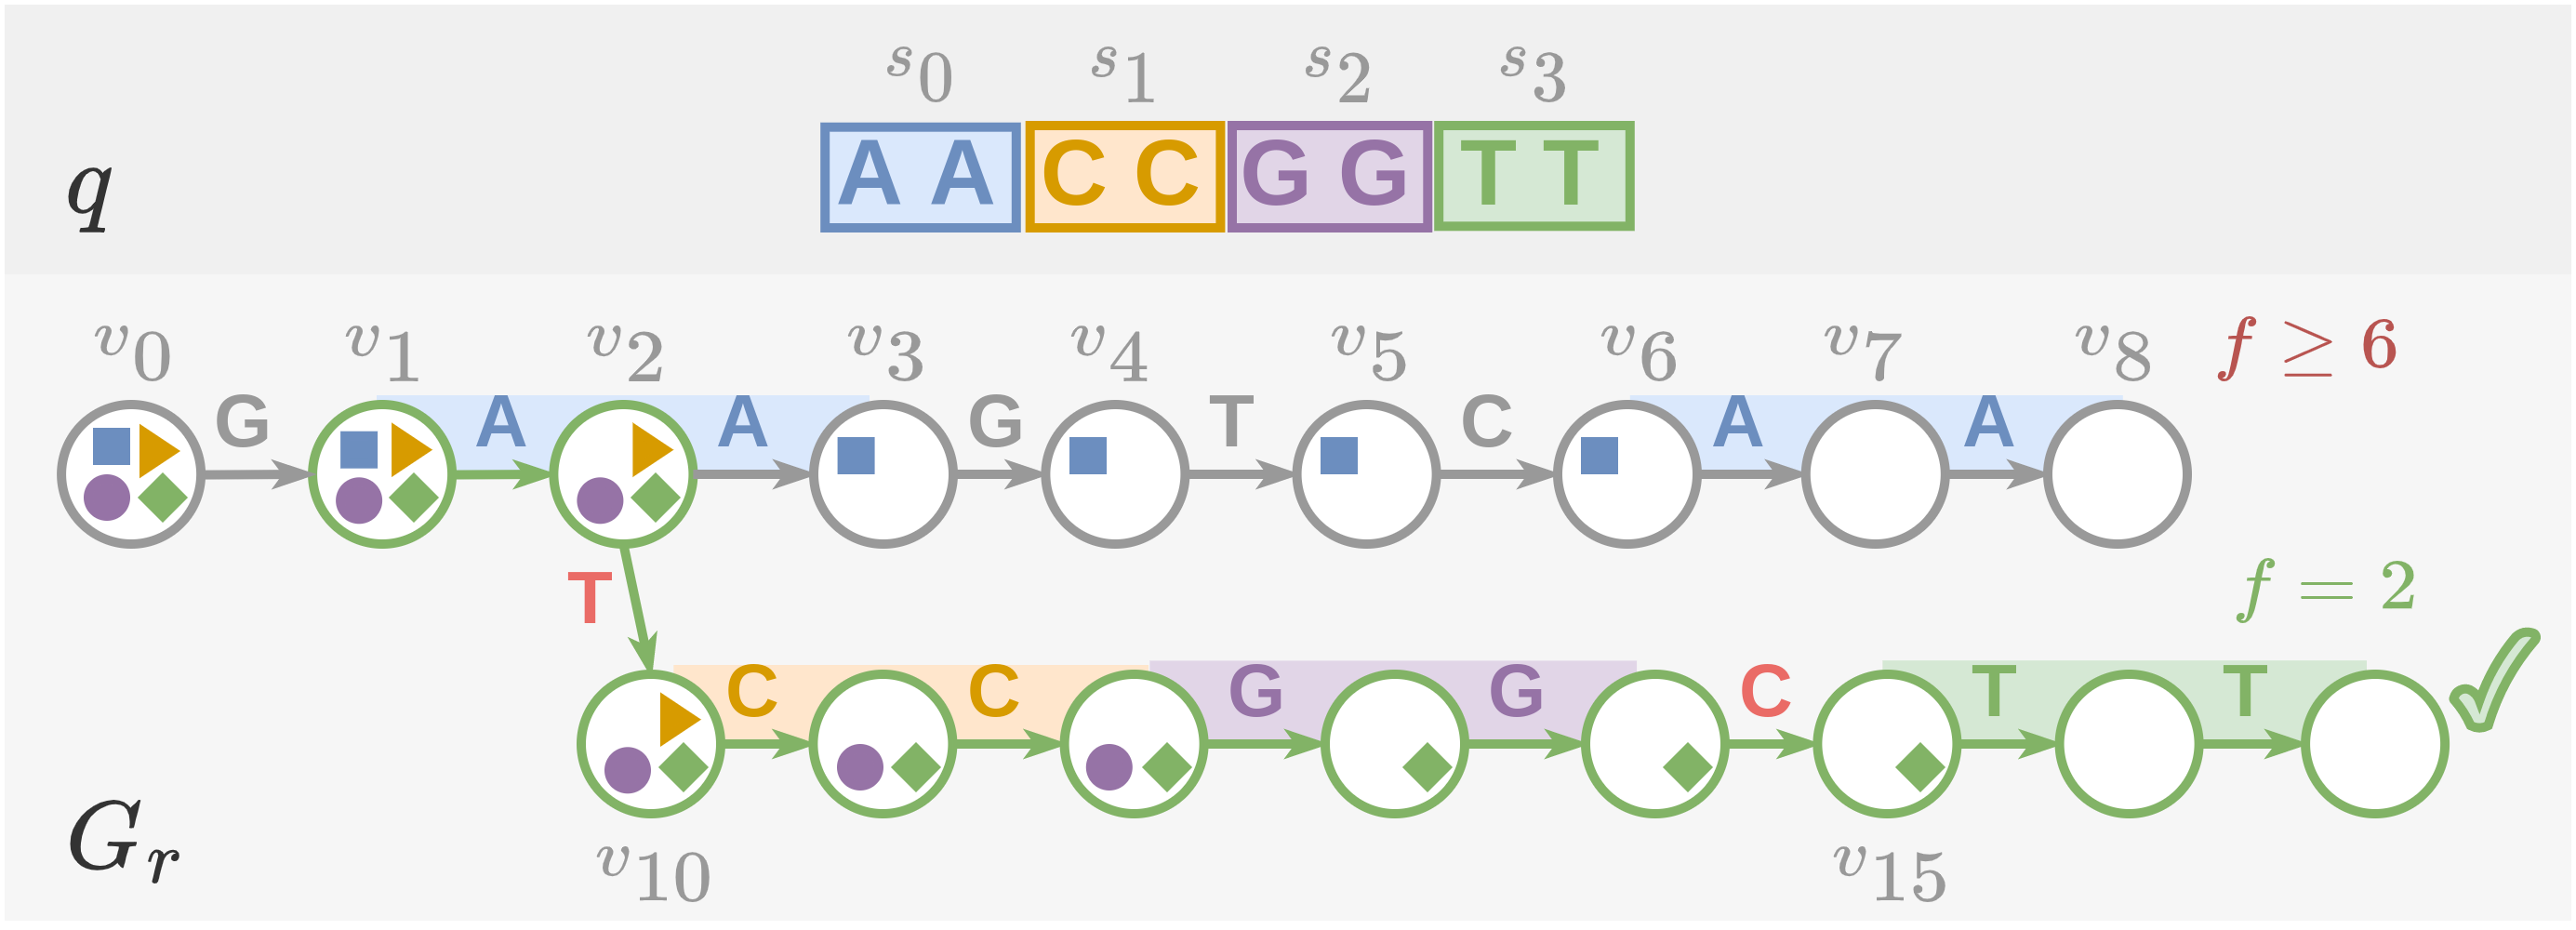
\includegraphics[width=0.8\linewidth]{figures/seed-heuristic-diagram.png}
	\caption[Seed heuristic precomputation: seeds, crumbs, matches]{%
		A toy illustration of the \seedh precomputation before aligning a read
		$q$ to a reference graph $\RG$. The read is split into four colored
		seeds, where their corresponding crumbs are shown inside reference graph
		nodes as symbols with matching color. The optimal alignment is
		highlighted as a green path ending with a tick (\protect\greentick{})
		and includes one substitution
		($\mathtt{\textcolor{dark-red}{T}{\rightarrow}\textcolor{dark-red}{A}}$)
		and one deletion ($\textcolor{dark-red}{\mathtt{C}}$).
		%
	}
\label{SEEDfig:overview}
\end{figure}